\section{Pianificazione}
\subsection{Analisi}
Questa fase ha inizio il 2015-12-17 e termina il 2016-01-18, prima della data di consegna per la \textit{Revisione dei Requisiti} in modo da poter contare su 4 giorni di \textit{slack}, dunque la ndurata del periodo ammonta a 32 giorni.

I ruoli attivi sono quelli di \textit{Amministratore}, \textit{Analista}, \textit{Responsabile}, \textit{Progettista} e \textit{Verificatore}.

La suddivisione in task \`e incentrata sull'\textit{Analisi dei requisiti}. Per tale motivo viene redatta e verificata prima di tutto la parte del \textit{Piano di progetto} relativa all'analisi. Seguendo la prassi del modello incrementale, alla conclusione di ogni stesura segue un periodo di verifica per ottenere una baseline non corrotta.
\subsubsection{Diagramma di Gantt}
\begin{figure}[ht!]
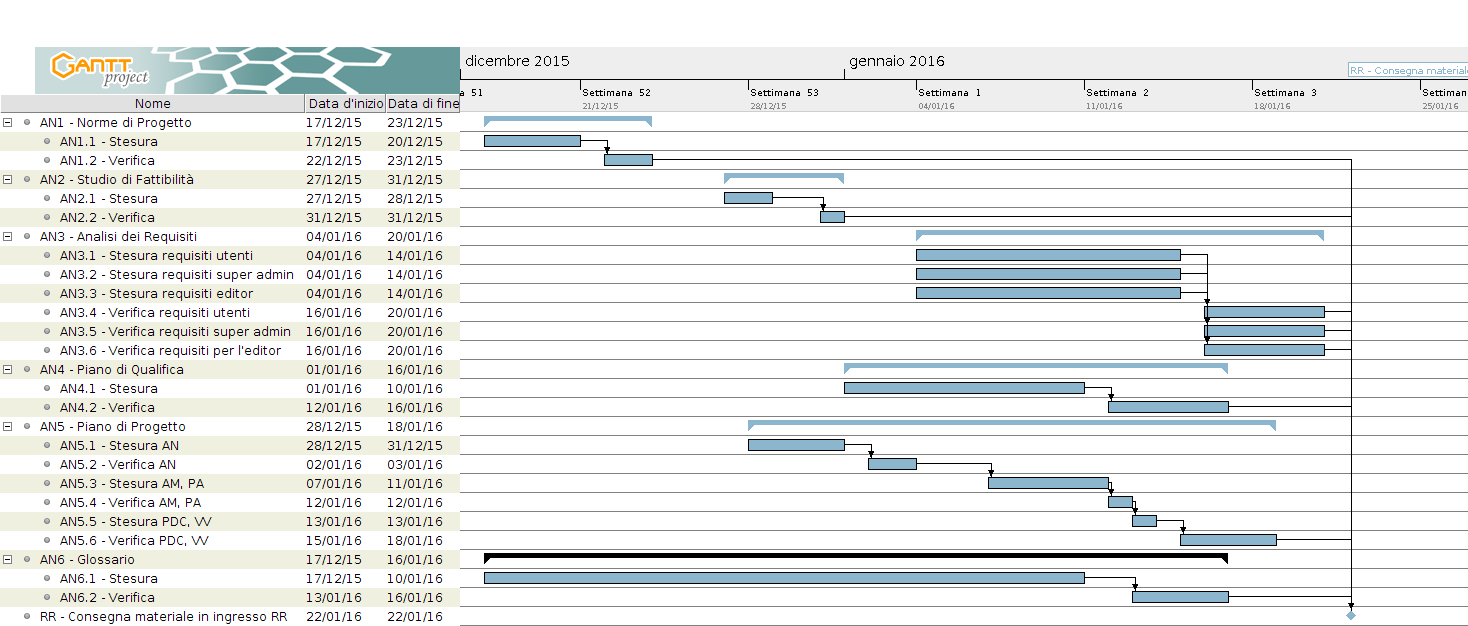
\includegraphics[width=1\textwidth]{res/img/PianoDiProgetto/Analisi.png}
\caption{Diagramma di Gantt, periodo di Analisi}
\end{figure}

\subsubsection{Ripartizione ore}

\begin{table}[H]
	\centering
	\begin{tabular*}{1\textwidth}{ @{\extracolsep{\fill} } l l l c  }
	\hline
	\multicolumn{1}{c}{\textbf{Id}} & 
	\multicolumn{1}{c}{\textbf{Nome}} & 
	\multicolumn{1}{c}{\textbf{Ruolo}}& 
	\multicolumn{1}{c}{\textbf{Ore}} \\
	\hline
	
	\textbf{AN1} & \textbf{Norme di progetto} \\
	\cline{3-4}
	AN1.1 & Stesura & Amministratore & 8\\ 
    & & Amministratore & 6\\
    & & Responsabile & 4 \\
    \cline{3-4}
	AN1.2 & Verifica & Verificatore & 4\\
	
	\hline
	\textbf{AN2} & \textbf{Studio di fattibilità} \\
	\cline{3-4}
	AN2.1 & Stesura & Analista & 3\\ 
    & & Analista & 3\\
    \cline{3-4}
	AN2.2 & Verifica & Verificatore &  1\\
	
	\hline
	\textbf{AN3} & \textbf{Piano di progetto} \\
	\cline{3-4}
	AN3.1 & Stesura AN & Amministratore & 2\\ 
    & & Responsabile & 8\\
    & & Responsabile & 8\\
    \cline{3-4}
	AN3.2 & Verifica AN & Verificatore & 3\\
	\cline{3-4}
	AN3.3 & Stesura AM, PA & Amministratore & 8\\ 
    & & Responsabile & 10\\
	\cline{3-4}
	AN3.4 & Verifica AM, PA & Verificatore & 2\\
	\cline{3-4}
	AN3.5 & Stesura PDC, VV & Amministratore & 4\\ 
        & & Responsabile & 3\\
	\cline{3-4}
	AN3.6 & Verifica PDC, VV & Verificatore & 2\\
	& & Verificatore & 2\\
	

	\hline
	\textbf{AN4} & \textbf{Analisi dei requisiti} \\
	\cline{3-4}
	AN4.1 & Stesura requisiti utenti & Analista1 & 11\\ 
    & & Analista2 & 5\\
    \cline{3-4}
	AN4.2 & Stesura requisiti super admin & Analista &  11\\
	\cline{3-4}
	AN4.3 & Stesure requisiti editor & Analista1 & 11\\ 
    & & Analista2 & 6\\
	\cline{3-4}
	AN4.4 & Verifica requisiti utenti & Verificatore &  4\\
        \cline{3-4}
        AN4.5 & Verifica requisiti super admin & Verificatore &  3\\
        \cline{3-4}
        AN4.6 & Verifica requisiti per l'editor & Verificatore &  3\\
        \hline
        \textbf{AN5} & \textbf{Piano di qualifica} \\
	\cline{3-4}
	AN5.1 & Stesura & Progettista & 4\\
	& & Progettista & 4\\
        & & Verificatore & 3\\
        \cline{3-4}
	AN5.2 & Verifica & Verificatore1 & 4\\
	& & Verificatore2 & 2\\
        \hline
	\end{tabular*}
	\end{table}

\begin{table}[H]
	\centering
	\begin{tabular*}{1\textwidth}{ @{\extracolsep{\fill} } l l l c  }
	\hline
	\multicolumn{1}{c}{\textbf{Id}} & 
	\multicolumn{1}{c}{\textbf{Nome}} & 
	\multicolumn{1}{c}{\textbf{Ruolo}}& 
	\multicolumn{1}{c}{\textbf{Ore}} \\
	\hline
	\textbf{AN6} & \textbf{Glossario} \\
	\cline{3-4}
	AN6.1 & Stesura & Amministratore & 5\\
        \cline{3-4}
	AN6.2 & Verifica & Verificatore & 3\\
	
	\hline
	\end{tabular*}
	\caption{Allocazione risorse, periodo di Analisi}
	\end{table}

\newpage

\subsection{Analisi Miglioramenti}
Questo periodo ha inizio il 2016-02-17 e termina il 2016-02-26, prima dell'inizio stabilito del PA, per un totale di 9 giorni.


I ruoli attivi sono quelli di \textit{Amministratore}, \textit{Progettista}, \textit{Validatore}, \textit{Programmatore}, \textit{Responsabile}.


Lo scopo di questo periodo \`e il consolidamento, il miglioramento e il cambiamento, se necessario, degli strumenti di supporto al progetto.\\
I membri del gruppo che occuperanno il ruolo di \textit{Amministratore} e \textit{Responsabile} saranno tenuti a ricercare strumenti alternativi ritenuti pi\`u validi rispetto a quelli adottati finora.\\
Il \textit{Validatore} dovr\`a occuparsi di verificare la qualit\`a di quest'ultimi al fine di non incontrare, durante le fasi successive, prodotti non conformi ai livelli stabiliti dal \textit{Piano di Qualifica} dovuti a cattiva strumentazione.\\
Infine, il \textit{Programmatore} affiancato dal \textit{Progettista} avr\`a il compito di allestire l'ambiente di lavoro.

\subsubsection{Diagramma di Gantt}
\begin{figure}[ht!]
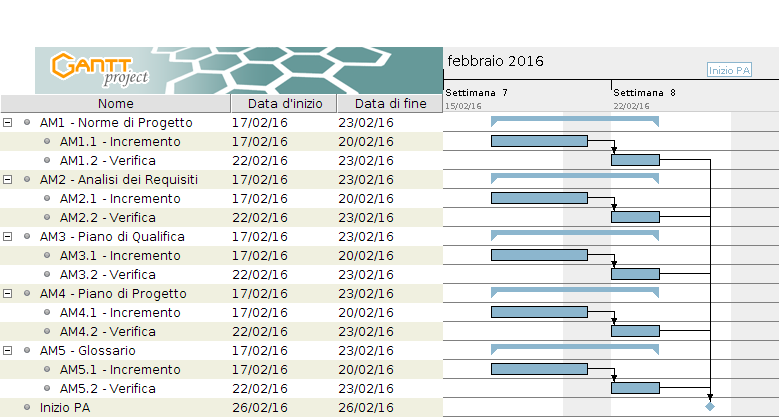
\includegraphics[width=1\textwidth]{res/img/PianoDiProgetto/AnalisiMiglioramenti.png}
\caption{Diagramma di Gantt, periodo di Analisi Miglioramenti}
\end{figure}


\subsubsection{Ripartizione ore}

\begin{table}[H]
	\centering
	\begin{tabular*}{1\textwidth}{ @{\extracolsep{\fill} } l l l c  }
	\hline
	\multicolumn{1}{c}{\textbf{Id}} & 
	\multicolumn{1}{c}{\textbf{Nome}} & 
	\multicolumn{1}{c}{\textbf{Ruolo}}& 
	\multicolumn{1}{c}{\textbf{Ore}} \\
	\hline
	
	\textbf{AM1} & \textbf{Norme di progetto} \\
	\cline{3-4}
	AM1.1 & Incremento & Amministratore & 4\\ 
    \cline{3-4}
	AM1.2 & Verifica & Verificatore & 2\\
	
	\hline
	\textbf{AM2} & \textbf{Analisi dei Requisiti} \\
	\cline{3-4}
	AM2.1 & Incremento & Analista & 4\\ 
        \cline{3-4}
	AM2.2 & Verifica & Verificatore & 2\\

        \hline
	\textbf{AM3} & \textbf{Piano di Qualifica} \\
	\cline{3-4}
	AM3.1 & Incremento & Verificatore & 1\\
        & & Progettista & 3\\
        \cline{3-4}
	AM3.2 & Verifica & Verificatore & 2\\
        
	\hline
	\textbf{AM4} & \textbf{Piano di Progetto} \\
	\cline{3-4}
	AM4.1 & Incremento & Responsabile & 1\\ 
        & & Amministratore & 3\\
    \cline{3-4}
	AM4.2 & Verifica AN & Verificatore & 2\\

	\hline
	\textbf{AM5} & \textbf{Glossario} \\
	\cline{3-4}
	AM5.1 & Incremento & Amministratore & 2\\ 
        & & Amministratore & 2\\
        \cline{3-4}
	AM5.2 & Verifica & Verificatore & 2\\

        \hline
	\end{tabular*}
        \caption{Allocazione risorse, periodi di Analisi Miglioramenti}
	\end{table}

\newpage

\subsection{Progettazione Architetturale}
Questa fase ha inizio il 2016-02-27 e termina 2016-04-11 per un totale di 45 giorni.

I ruoli attivi sono quelli di \textit{Amministratore}, \textit{Analista}, \textit{Responsabile}, \textit{Progettista} e \textit{Verificatore}.

Si suddivide la progettazione architetturale in progettazione dei requisiti fondamentali e desiderabili e progettazione dei requisiti opzionali. Inoltre, rimane attiva la stesura e verifica dei documenti scritti precedentemente, per tutte le aggiunte e i miglioramenti emersi durante la progettazione architetturale.

\subsubsection{Diagramma di Gantt}
\begin{figure}[ht!]
  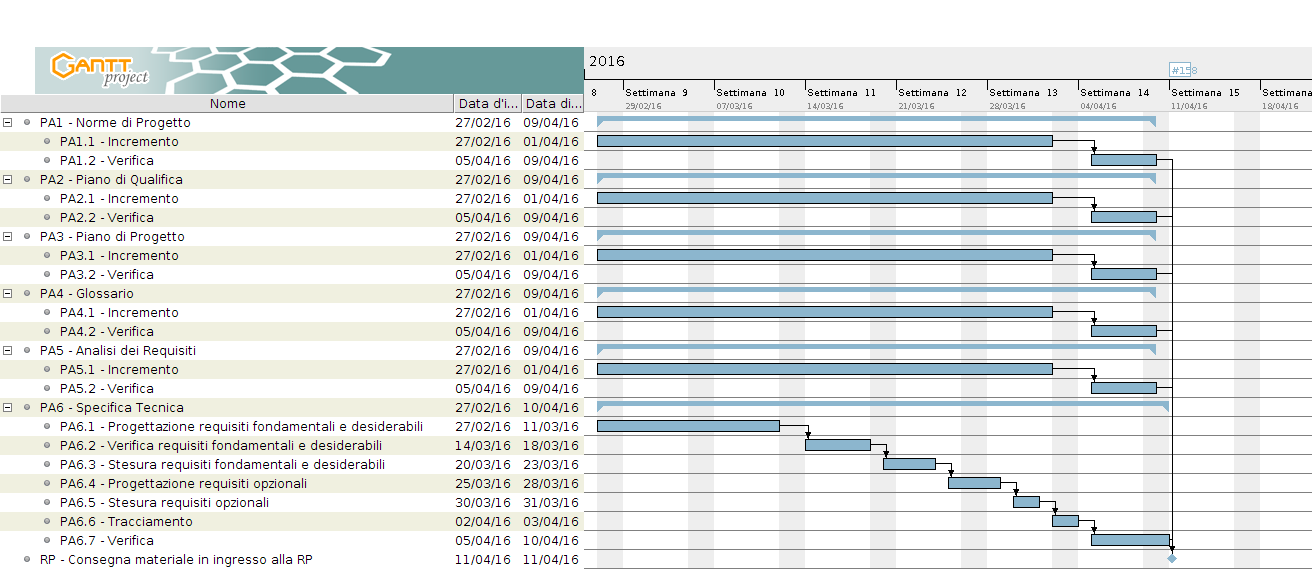
\includegraphics[width=1\textwidth]{res/img/PianoDiProgetto/ProgettazioneArchitetturale}
  \caption{Diagramma di Gantt, periodo Progettazione Architetturale}
\end{figure}

\subsubsection{Ripartizione ore}
\begin{table}[H]
	\centering
	\begin{tabular*}{1\textwidth}{ @{\extracolsep{\fill} } l l l c  }
	\hline
	\multicolumn{1}{c}{\textbf{Id}} & 
	\multicolumn{1}{c}{\textbf{Nome}} & 
	\multicolumn{1}{c}{\textbf{Ruolo}}& 
	\multicolumn{1}{c}{\textbf{Ore}} \\
	\hline
	
	\textbf{PA1} & \textbf{Norme di progetto} \\
	\cline{3-4}
	PA1.1 & Incremento & Amministratore & 2\\ 
        \cline{3-4}
	PA1.2 & Verifica & Verificatore & 1\\
	
	\hline
	\textbf{PA2} & \textbf{Piano di Qualifica} \\
	\cline{3-4}
	PA2.1 & Incremento & Verificatore & 3\\ 
        & & Verificatore & 2\\
        & & Progettista & 2 \\
        \cline{3-4}
	PA2.2 & Verifica & Verificatore &  3\\
	
	\hline
	\textbf{PA3} & \textbf{Piano di progetto} \\
	\cline{3-4}
	PA3.1 & Incremento & Responsabile & 2\\ 
        \cline{3-4}
	PA3.2 & Verifica & Verificatore & 1\\

	\hline
	\textbf{PA4} & \textbf{Glossario} \\
	\cline{3-4}
	PA4.1 & Incremento & Amministratore & 3\\ 
        & & Amministratore & 3\\
        \cline{3-4}
	PA4.2 & Verifica & Verificatore & 2\\
        & & Verificatore & 2\\

        \hline
        \textbf{PA5} & \textbf{Analisi Requisiti}\\
        \cline{3-4}
        PA5.1 & Incremento & Analista & 3\\
        \cline{3-4}
        PA5.2 & Verifica & Verificatore & 2\\
        & & Verificatore & 2\\
        
        \hline
        \textbf{PA6} & \textbf{Specifica Tecnica} \\
	\cline{3-4}
	PA6.1 & Progettazione requisiti fondamentali e desiderabili & Progettista & 19\\ 
        & & Progettista & 19\\
        & & Progettista & 19\\
        \cline{3-4}
	PA6.2 & Verifica requisiti fondamentali e desiderabili & Verificatore & 13\\
        & & Verificatore & 13\\
        \cline{3-4}
	PA6.3 & Stesura requisiti fondamentali e desiderabili & Progettista & 5\\
        & & Progettista & 4\\
        & & Progettista & 4\\
        & & Progettista & 4\\
        \cline{3-4}
	PA6.4 & Progettazione requisiti opzionali & Progettista & 8\\
        & & Progettista & 9\\
        & & Progettista & 9\\
        & & Progettista & 9\\

        \hline
        \end{tabular*}
\end{table}

\newpage

\begin{table}[H]
	\centering
	\begin{tabular*}{1\textwidth}{ @{\extracolsep{\fill} } l l l c  }
	\hline
	\multicolumn{1}{c}{\textbf{Id}} & 
	\multicolumn{1}{c}{\textbf{Nome}} & 
	\multicolumn{1}{c}{\textbf{Ruolo}}& 
	\multicolumn{1}{c}{\textbf{Ore}} \\

        \hline
	PA6.5 & Stesura requisiti opzionali & Progettista & 3\\
        & & Progettista & 3\\
        & & Progettista & 2\\
        & & Progettista & 2\\
        \cline{3-4}
	PA6.6 & Tracciamento & Progettista & 5\\
        & & Progettista & 5\\
        & & Progettista & 5\\
        & & Progettista & 5\\
        \cline{3-4}
	PA6.7 & Verifica & Verificatore & 8\\
        & & Verificatore & 8\\
        & & Verificatore & 7\\
        & & Verificatore & 7\\
        \hline
	\end{tabular*}
        \caption{Allocazione risorse, periodo di Progettazione Architetturale}
	\end{table}

\newpage

\subsection{Progettazione di Dettaglio e Codifica}
Questa fase ha inizio il 2016-04-19 e termina il 2016-05-14 per un totale 30 giorni.

I ruoli attivi in questa fase sono quello di \textit{Amministratore}, \textit{Progettista}, \textit{Programmatore}, \textit{Responsabile}, \textit{Verificatore}.

Oltre agli incrementi presenti per mantenere aggiornati i documenti, in questa fase si pianifica la realizzazione del prodotto completo che soddisfi i requisiti fondamentali, desiderabili ed opzionali. Una volta avvenuta la verifica su tutta la progettazione, si effettua la codifica e la stesura del manuale dell'utente da consegnare al proponente come verifica dei requisiti richiesti e la qualit\`a fissata.

\subsubsection{Diagramma di Gantt}
\begin{figure}[ht!]
  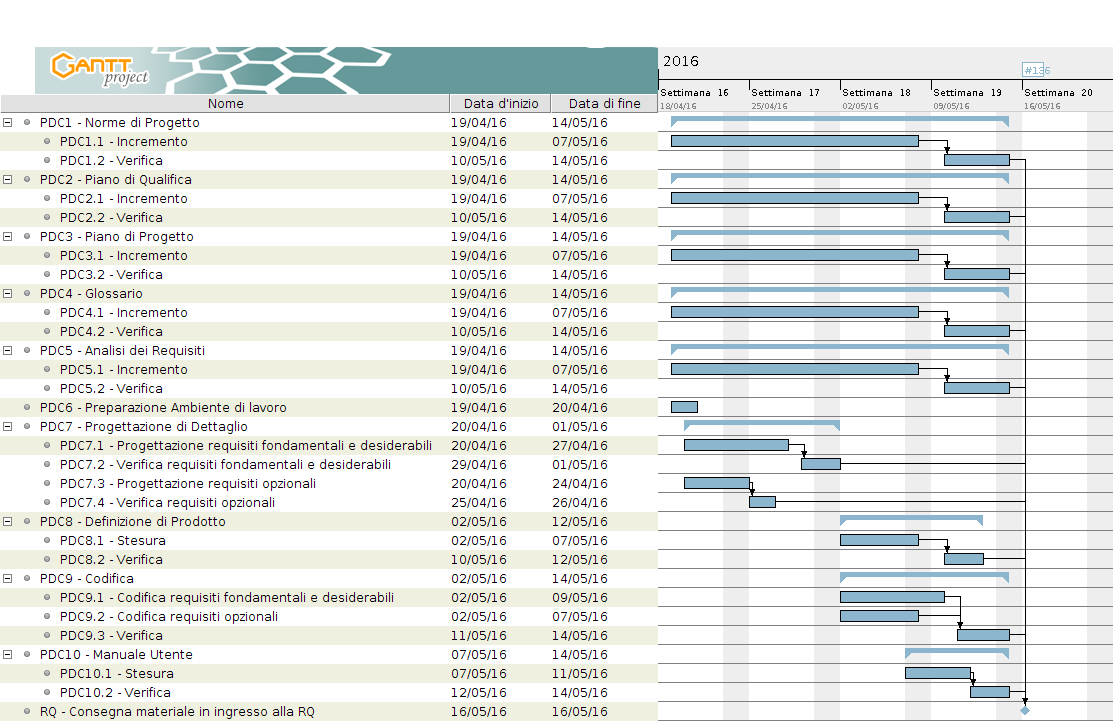
\includegraphics[width=1\textwidth]{res/img/PianoDiProgetto/ProgettazioneDettaglioECodifica.png}
  \caption{Diagramma di Gantt, periodo Progettazione di Dettaglio e Codifica}
\end{figure}

\subsubsection{Ripartizione orario}
\begin{table}[H]
	\centering
	\begin{tabular*}{1\textwidth}{ @{\extracolsep{\fill} } l l l c  }
	\hline
	\multicolumn{1}{c}{\textbf{Id}} & 
	\multicolumn{1}{c}{\textbf{Nome}} & 
	\multicolumn{1}{c}{\textbf{Ruolo}}& 
	\multicolumn{1}{c}{\textbf{Ore}} \\
	\hline
	
	\textbf{PDC1} & \textbf{Norme di progetto} \\
	\cline{3-4}
	PA1.1 & Incremento & Amministratore & 3\\ 
        \cline{3-4}
	PDC1.2 & Verifica & Verificatore & 1\\
	
	\hline
	\textbf{PDC2} & \textbf{Piano di Qualifica} \\
	\cline{3-4}
	PDC2.1 & Incremento & Progettista & 4\\
        & & Verificatore & 2\\
        \cline{3-4}
	PDC2.2 & Verifica & Verificatore & 2\\
	
	\hline
	\textbf{PDC3}  & \textbf{Piano di progetto} \\
	\cline{3-4}
	PDC3.1 & Incremento & Responsabile & 3\\ 
        \cline{3-4}
	PDC3.2 & Verifica & Verificatore & 2\\

	\hline
	\textbf{PDC4} & \textbf{Glossario} \\
	\cline{3-4}
	PDC4.1 & Incremento & Amministratore & 3\\ 
        \cline{3-4}
	PDC4.2 & Verifica & Verificatore & 1\\

        \hline
        \textbf{PDC5} & \textbf{Analisi dei Requisiti}\\
        \cline{3-4}
        PDC5.1 & Incremento & Analista & 3\\
        \cline{3-4}
        PDC5.2 & Verifica & Verificatore 2\\

        \hline
        \textbf{PDC6} & \textbf{Preparazione Ambiente di lavoro} & Amministratore & 10\\

        \hline
        \textbf{PDC7} & \textbf{Progettazione di Dettaglio} \\
	\cline{3-4}
	PDC5.1 & Progettazione requisiti fondamentali e desiderabili & Progettista & 30\\ 
        & & Progettista & 9\\
        & & Progettista & 9\\
        \cline{3-4}
	PDC5.2 & Verifica requisiti fondamentali e desiderabili & Verificatore & 10\\
        \cline{3-4}
	PDC5.3 & Progettazione requisiti opzionali & Progettista & 15\\
        & & Progettista & 13\\
        \cline{3-4}
	PDC5.4 & Verifica requisiti opzionali & Verificatore & 5\\

        \hline
        \textbf{PDC7} & \textbf{Definizione di Prodotto} \\
	\cline{3-4}
	PDC7.1 & Stesura & Progettista & 40\\ 
        \cline{3-4}
        PDC7.2 & Verifica & Verifica & 7\\
        & & Verifica & 4\\

        \hline
        \end{tabular*}
\end{table}

\begin{table}[H]
	\centering
	\begin{tabular*}{1\textwidth}{ @{\extracolsep{\fill} } l l l c  }
	\hline
	\multicolumn{1}{c}{\textbf{Id}} & 
	\multicolumn{1}{c}{\textbf{Nome}} & 
	\multicolumn{1}{c}{\textbf{Ruolo}}& 
	\multicolumn{1}{c}{\textbf{Ore}} \\

        \hline

        \textbf{PDC8} & \textbf{Codifica} \\
	\cline{3-4}
	PDC8.1 & Codifica requisiti fondamentali e desiderabili & Programmatore & 31\\
        & & Programmatore & 30\\
        & & Programmatore & 8\\
        & & Programmatore & 8\\
        & & Programmatore & 8\\
        \cline{3-4}
	PDC8.2 & Codifica requisiti opzionali & Programmatore & 20\\
        & & Programmatore & 18\\
        & & Programmatore & 18\\
        \cline{3-4}
        PDC8.3 & Verifica & Verificatore & 9\\
        \hline
	\textbf{PDC8} & \textbf{Manuale Utente} \\
	\cline{3-4}
	PDC8.1 & Stesura & Amministratore & 34\\ 
        \cline{3-4}
	PDC8.2 & Verifica & Verificatore & 7\\
        & & Verificatore & 4\\
        \hline
	\end{tabular*}
        \caption{Allocazione risorse, periodo di Progettazione di Dettaglio e Codifica}
\end{table}

\newpage

\subsection{Verifica e Validazione}
Questo periodo ha inizio il 2016-05-24 e termina il 2016-06-09, per un totale di 16 giorni.
I ruoli attivi sono quello di \textit{Amministratore}, \textit{Progettista}, \textit{Responsabile}, \textit{Verificatore}.

Con l'adozione del modello incrementale il risultato \`e un ultimo momento molto breve in cui eseguire i test di sistema e rilasciare il prodotto completo per il collaudo dell'RA. Nello stesso momento vengono redatte le ultime versioni dei documenti da rilasciare alla commissione e al committente.

\subsubsection{Diagramma di Gantt}
\begin{figure}[ht!]
  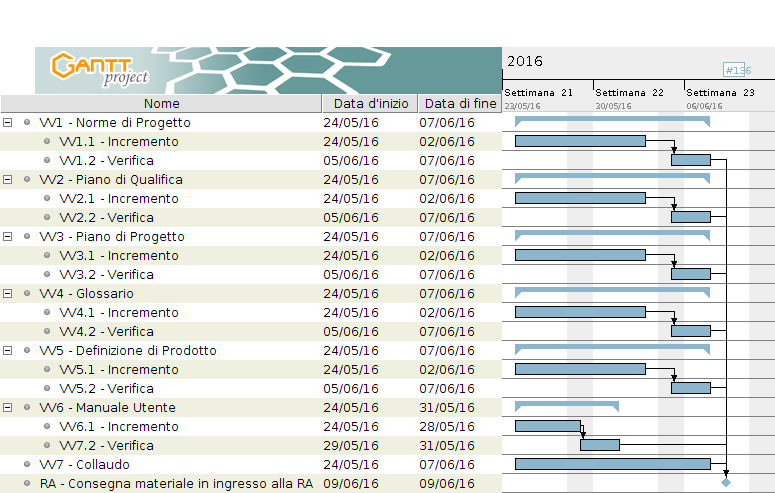
\includegraphics[width=1\textwidth]{res/img/PianoDiProgetto/VerificaEValidazione.png}
  \caption{Diagramma di Gantt, periodo di Verifica e Validazione}
\end{figure}

\subsubsection{Ripartizione orario}

\begin{table}[H]
	\centering
	\begin{tabular*}{1\textwidth}{ @{\extracolsep{\fill} } l l l c  }
	\hline
	\multicolumn{1}{c}{\textbf{Id}} & 
	\multicolumn{1}{c}{\textbf{Nome}} & 
	\multicolumn{1}{c}{\textbf{Ruolo}}& 
	\multicolumn{1}{c}{\textbf{Ore}} \\
	\hline
	
	\textbf{VV1} & \textbf{Norme di progetto} \\
	\cline{3-4}
	VV1.1 & Incremento & Amministratore & 2\\ 
    \cline{3-4}
	VV1.2 & Verifica & Verificatore & 2\\
	
	\hline
	\textbf{VV2} & \textbf{Piano di Qualifica} \\
	\cline{3-4}
	VV2.1 & Incremento & Verificatore & 2\\
        \cline{3-4}
	VV2.2 & Verifica & Verificatore & 2\\
	
	\hline
	\textbf{VV3} & \textbf{Piano di progetto} \\
	\cline{3-4}
	VV3.1 & Incremento & Responsabile & 1\\
        \cline{3-4}
	VV3.2 & Verifica & Verificatore & 2\\

	\hline
	\textbf{VV4} & \textbf{Glossario} \\
	\cline{3-4}
	VV4.1 & Incremento & Amministratore & 1\\
    \cline{3-4}
	VV4.2 & Verifica & Verificatore & 2\\

        \hline
        \textbf{VV5} & \textbf{Definizione di Prodotto} \\
	\cline{3-4}
        VV5.1 & Incremento & Progettista & 12\\
        \cline{3-4}
	VV5.2 & Verifica & Verificatore & 5\\

        \hline
        \textbf{VV6} & \textbf{Manuale Utente} \\
	\cline{3-4}
        VV5.1 & Incremento & Amministratore & 10\\
        \cline{3-4}
	VV5.2 & Verifica & Verificatore & 8\\
                
        \hline
        \textbf{VV7} & \textbf{Collaudo} & Verificatore & 15\\
        & & Verificatore & 15\\
        & & Verificatore & 10\\
        & & Verificatore & 7\\
        & & Verificatore & 5\\
        & & Programmatore & 5\\

        \hline
	\end{tabular*}
        \caption{Allocazione risorse, periodo di Verifica e Validazione}
	\end{table}



